\documentclass[10pt, serif, professionalfonts, usenames,dvipsnames]{beamer}

% There are many different themes available for Beamer. A comprehensive
% list with examples is given here:
% http://deic.uab.es/~iblanes/beamer_gallery/index_by_theme.html
% You can uncomment the themes below if you would like to use a different
% one:
%\usetheme{AnnArbor}
%\usetheme{Antibes}
%\usetheme{Bergen}
%\usetheme{Berkeley}
%\usetheme{Berlin}
%\usetheme{Boadilla}
%\usetheme{boxes}
%\usetheme{CambridgeUS}
%\usetheme{Copenhagen}
%\usetheme{Darmstadt}
\usetheme{default}
%\usetheme{Frankfurt}
%\usetheme{Goettingen}
%\usetheme{Hannover}
%\usetheme{Ilmenau}
%\usetheme{JuanLesPins}
%\usetheme{Luebeck}
%\usetheme{Madrid}
%\usetheme{Malmoe}
%\usetheme{Marburg}
%\usetheme{Montpellier}
%\usetheme{PaloAlto}
%\usetheme{Pittsburgh}
%\usetheme{Rochester}
%\usetheme{Singapore}
%\usetheme{Szeged}
%\usetheme{Warsaw}

\usepackage{tikz}
\usetikzlibrary{shadings}
\definecolor{secinhead}{RGB}{249,196,95}
\definecolor{shadowbg}{RGB}{51,51,51}
\usetikzlibrary{intersections}
\usepackage{pgfplots}
\pgfplotsset{compat=1.16}
\usepgfplotslibrary{fillbetween}
\tikzset{
	invisible/.style={opacity=0},
	visible on/.style={alt={#1{}{invisible}}},
	alt/.code args={<#1>#2#3}{%
		\alt<#1>{\pgfkeysalso{#2}}{\pgfkeysalso{#3}} % \pgfkeysalso doesn't change the path
	},
}


\setbeamercolor{secsubsec}{fg=secinhead,bg=black}
\setbeamercolor{shadow}{fg=secinhead,bg=shadowbg}


\setbeamertemplate{navigation symbols}{}

\usepackage{amsmath}
\usepackage{amsfonts}
\usepackage{amsthm}
\usepackage{amssymb}
\usepackage{commath}
\usepackage[utf8]{inputenc}
\usepackage[english]{babel}
%\usepackage[authoryear]{natbib}  % 

\usepackage{graphicx}
\DeclareGraphicsRule{.ai}{pdf}{.ai}{} 
\usepackage{epstopdf}
\usepackage{bm}
\usepackage{multirow}

\usepackage{tikz}
\usetikzlibrary{arrows,shapes}
\usetikzlibrary{positioning,arrows.meta}

\usepackage{longtable}
\usepackage{booktabs}
\usepackage{adjustbox}
\usepackage{geometry}
\usepackage{graphics}
\usepackage{multimedia} % for movies and sound
\usepackage{times}
\usepackage{xcolor,colortbl}
%\definecolor{green}{rgb}{0.1,0.1,0.1}
\newcommand{\done}{\cellcolor{teal}done}  %{0.9}
\newcommand{\hcyan}[1]{{\color{teal} #1}}
\usepackage{caption}
\usepackage{subcaption}
%\usepackage{subfig}

\usepackage{listings}
%\usepackage[usenames,dvipsnames]{color}    
\lstset{ 
	language=R,                     % the language of the code
	basicstyle=\scriptsize\ttfamily, % the size of the fonts that are used for the code
	numbers=left,                   % where to put the line-numbers
	numberstyle=\scriptsize\color{Blue},  % the style that is used for the line-numbers
	stepnumber=1,                   % the step between two line-numbers. If it is 1, each line
	% will be numbered
	numbersep=5pt,                  % how far the line-numbers are from the code
	backgroundcolor=\color{gray!05},  % choose the background color. You must add \usepackage{color}
	showspaces=false,               % show spaces adding particular underscores
	showstringspaces=false,         % underline spaces within strings
	showtabs=false,                 % show tabs within strings adding particular underscores
	frame=single,                   % adds a frame around the code
	rulecolor=\color{black},        % if not set, the frame-color may be changed on line-breaks within not-black text (e.g. commens (green here))
	tabsize=2,                      % sets default tabsize to 2 spaces
	captionpos=b,                   % sets the caption-position to bottom
	breaklines=true,                % sets automatic line breaking
	breakatwhitespace=false,        % sets if automatic breaks should only happen at whitespace
	keywordstyle=\color{RoyalBlue},      % keyword style
	commentstyle=\color{YellowGreen},   % comment style
	stringstyle=\color{ForestGreen}      % string literal style
} 

%\newtheorem{theorem}{Theorem}[section]
%\newtheorem{corollary}{Corollary}[theorem]
%\newtheorem{lemma}[theorem]{Lemma}

%algorithm
\providecommand{\tabularnewline}{\\}
%\floatstyle{ruled}
%\newfloat{algorithm}{tbp}{loa}
\providecommand{\algorithmname}{Algorithm}
%\floatname{algorithm}{\protect\algorithmname}

% NEWCOMMANDS
\newcommand{\loss}{\ensuremath{l}}
\newcommand{\response}{\ensuremath{y}}
\newcommand{\features}{\ensuremath{\mathbf{x}}}
\newcommand{\pred}{\ensuremath{\hat{y}}}
\newcommand{\data}{\ensuremath{\mathcal{D}}}
%\newcommand{\E}{\ensuremath{\mathbb{E}}}
\newcommand{\E}{\ensuremath{E}}
\newcommand{\Var}{\mathrm{Var}}
\newcommand{\Cov}{\mathrm{Cov}}
\newcommand{\tr}{\mathrm{tr}}
\newcommand{\Prob}{\ensuremath{\mathbb{P}}}
\newcommand{\setleafnodes}{\ensuremath{\mathcal{L}}}

\usepackage{mathtools}
\DeclarePairedDelimiter{\ceil}{\lceil}{\rceil}

\usepackage{lmodern}
\setbeamertemplate{blocks}[shadow=false]
%\beamertemplatenavigationsymbolsempty
\usecolortheme{rose}
\useinnertheme{circles}

\newenvironment{myblock}[3]{%
	\setbeamercolor{block body}{#2}
	\setbeamercolor{block title}{#3}
	\begin{block}{#1}}{\end{block}}

%\setbeamercovered{dynamic}


%\title{Adaptive computations in gradient tree boosting}
\title{An information criterion for gradient boosted trees}
%\subtitle{Adaptive tree-size and early stopping}


\author{Berent Ånund Strømnes Lunde\inst{1} \\
	\and Tore Selland Kleppe\inst{1} \and Hans Julius Skaug\inst{2}}
% - Give the names in the same order as the appear in the paper.
% - Use the \inst{?} command only if the authors have different
%   affiliation.

\institute[]
{
	\inst{1}   
	Department of Mathematics and Physics\\
	University of Stavanger
	\and
	\inst{2}
	Department of Mathematics\\
	University of Bergen
}
% - Use the \inst command only if there are several affiliations.
% - Keep it simple, no one is interested in your street address.

% logo of my university
%\titlegraphic{\includegraphics[height=1.4cm]{figures/UiS_main_logo_positive_CMYK_English.ai}}

\date{BigInsight - Wednesday Lunch\\
	UiO, Oslo\\
	9th October 2019}
% - Either use conference name or its abbreviation.
% - Not really informative to the audience, more for people (including
%   yourself) who are reading the slides online


% the beginning of each subsection:
\AtBeginSection{
\begin{frame}
	\tableofcontents[currentsection]
\end{frame}
}

%\AtBeginSubsection[]
%{
%  \begin{frame}<beamer>{Outline}
%    \tableofcontents[currentsection,currentsubsection]
%  \end{frame}
%}

% Let's get started
\begin{document}	
	
\tikzstyle{every picture}+=[remember picture]
	
\addtobeamertemplate{frametitle}{}{%

\begin{tikzpicture}[remember picture,overlay]
	\tikz\draw[draw=none,top color=gray,bottom color=shadowbg!10] (1,0) rectangle (1.1\paperwidth,0.1);
	%\node[anchor=south west,yshift=0pt, xshift=3pt] at (current page.south west){\includegraphics[height=1.4cm]{figures/UiS_main_logo_positive_CMYK_English.ai}};
	\node[anchor=south, yshift=0pt, xshift=4pt] at (current page.south){\small{\textcolor{black}{Berent Å. S. Lunde}    \textcolor{brown}{An information criterion for gradient boosted trees}}};
\end{tikzpicture}}

\begin{frame}
  \titlepage
\end{frame}

\begin{frame}
	\frametitle{Outline}
	\tableofcontents
\end{frame}


\section{Background}

%\subsection{Supervised learning and gradient tree boosting}

\begin{frame}{Question 1: Linear regression}
	
	\begin{columns}[T]
		\begin{column}{0.35\textwidth}
			%\begin{figure}
				\includegraphics<1->[height=2.9cm,width=3.5cm]{figures/growth_girls_lm.pdf} 
				\includegraphics<1->[height=2.9cm,width=3.5cm]{figures/growth_boys_lm.pdf}		
			%\end{figure}
		\end{column}
		\begin{column}{0.6\textwidth}
			\begin{myblock}{Researcher asks...}{bg=blue!5,fg=black}{bg=blue!10, fg=black}
				How can I model the \textcolor{orange}{\texttt{height}} of children given their \textcolor{orange}{\texttt{age}} and \textcolor{orange}{\texttt{sex}}?
				And I need a model fast! [Berkeley growth curve dataset]
			\end{myblock}
		\visible<2>{
			\begin{myblock}{The statistician responds...}{bg=yellow!05,fg=black}{bg=yellow!20, fg=black}
				Easy! Just try a linear regression: 
				$\textcolor{orange}{\texttt{height}}\approx \beta_0 + \beta_1 
				\textcolor{orange}{\texttt{age}} + \beta_2 \textcolor{orange}{\texttt{sex}}$.
				Estimate parameters $\mathbf{\beta} = \{\beta_0, \beta_1, \beta_2\}$ by minimizing the mean squared error (MSE):\\ $\hat{\mathbf{\beta}} = \arg\min_\mathbf{\beta} \sum_i \left(y_i - f(\textcolor{orange}{\texttt{age}}_i,\textcolor{orange}{\texttt{sex}}_i;\mathbf{\beta})\right)^2$.
			\end{myblock}}
		\end{column}
	\end{columns}
	
\end{frame}

\begin{frame}{Question 2: Generalized linear models}
	
	\begin{columns}[T]
	\begin{column}{0.35\textwidth}
		%\begin{figure}
		\includegraphics<1->[height=5.5cm,width=4cm]{figures/claims_glm.pdf} 
		%\includegraphics<1->[height=2.9cm,width=3.5cm]{figures/growth_boys_lm.pdf}		
		%\end{figure}
	\end{column}
	\begin{column}{0.6\textwidth}
		\begin{myblock}{Researcher asks...}{bg=blue!5,fg=black}{bg=blue!10, fg=black}
			Is there an efficient way to model the \textcolor{orange}{\texttt{risk}} of customers of insurance given some history of \textcolor{orange}{\texttt{claims}} and information about the customers?
			The model needs to be production friendly!
		\end{myblock}
		\visible<2>{
			\begin{myblock}{The actuary responds...}{bg=yellow!05,fg=black}{bg=yellow!20, fg=black}
				Easy! Divide and conquer: split the \textcolor{orange}{\texttt{claims}} into \textcolor{orange}{\texttt{size}} and \textcolor{orange}{\texttt{frequency}} and model them using a gamma and a Poisson generalized linear model, respectively. The \texttt{glm()}-function in R is your friend.
		\end{myblock}}
	\end{column}
\end{columns}
 
\end{frame}


\begin{frame}{Supervised learning}
	
	\begin{itemize}
		\item The above problems may be framed as \textcolor{orange}{supervised learning}:
	\end{itemize}
	
	\begin{block}{Supervised learning}
		Find the best (in expectation, relative to loss $l$) predictive function:
		\begin{align*}
		\hat{f} = \arg\min_f E_{\features\response}\left[l(\response,f(\features))\right]
		\end{align*}
		The loss often correspond to a nll.
\end{block}

\visible<2->{
\begin{myblock}{User restricted $f$, is it...}{bg=yellow!05,fg=black}{bg=yellow!20, fg=black}
	\begin{itemize}
		\item Non-linear?
		\item Continuous?
		\item Which features should it use?
		\item Do we have enough data to parametrize $f$?
	\end{itemize}}
\end{myblock}
	
	
	
%	\begin{columns}[T]
%		\begin{column}{0.52\textwidth}
%			\begin{block}{Maximum likelihood}
%				LR and GLM both learn their parameters from data:%, by maximizing the likelihood of observing the data, given that the data was generated by the model.
%				\begin{align*}
%					\hat{\beta} = \arg\max_\beta p(\texttt{data}|\beta)
%				\end{align*}
%				\visible<2->{
%				Equivalent to minimizing the nll
%				\begin{align*}
%					\hat{\beta} = \arg\min_\beta \left\{- \sum_i \log (p(\texttt{obs}_i|\beta))\right\}
%				\end{align*}
%				assuming independent observations
%				\begin{itemize}
%					\item Minimizing MSE correspond to minimizing a Gaussian nll.
%				\end{itemize}}
%			\end{block}
%		\end{column}
%		\begin{column}{0.5\textwidth}
%			\visible<3->{
%			\begin{block}{Supervised learning}
%				Find the best (in expectation, relative to loss $l$) predictive function:
%				\begin{align*}
%					\hat{f} = \arg\min E_{\features\response}\left[l(\response,f(\features))\right]
%				\end{align*}
%				
%				The loss often correspond to a nll.
%				\visible<4->{
%				User restricted $f$: 
%				Is it
%				\begin{itemize}
%					\item Non-linear?
%					\item Continuous?
%					\item Which features should it use?
%					\item Do we have enough data to parametrize $f$?
%				\end{itemize}}
%			\end{block}}
%		\end{column}
%	\end{columns}
	
	
	
\end{frame}


\begin{frame}{Question 3: Gradient boosting}
	
	
	\begin{myblock}{Researcher asks...}{bg=blue!5,fg=black}{bg=blue!10, fg=black}
		I want to do well in this ML-competition, but...
		\begin{itemize}
			\item<2-> My data has missing values
			\item<2-> Both $n$ and $p$ are very large (design matrix with some billion elements)
			\item<2-> Relationships are non-linear and possibly discontinuous
			\item<2-> I don't care about explainability, just give me predictive power!
		\end{itemize}
	\end{myblock}
	\visible<3->{\begin{myblock}{The data scientist/Kaggle master responds...}{bg=yellow!05,fg=black}{bg=yellow!20, fg=black}
		Try gradient boosting? 
		\begin{itemize}\small
			\item<3-> State-of-the-art gradient boosting libraries: XGBoost, LightGBM and CatBoost.
		\end{itemize}
	\end{myblock}}

\end{frame}

\begin{frame}{Gradient boosting, what is going on behind the scenes?}
	
	Gradient boosting attacks the supervised learning problem directly
	
	%For many problems coined as supervised learning problems, gradient boosting
	
	\begin{myblock}{}{bg=blue!5,fg=black}{bg=blue!10, fg=black}
		\begin{itemize}
			\item Start with a constant value: $f^{(0)} = \arg\min_\eta \sum_i l(y_i,\eta)$
			\item Iteratively, add $\delta f_k$ to $f^{(k-1)}$, where $f_k$ is trained on the "error" (MSE case) of $f^{(k-1)}$, and $\delta$ is some small number scaling $f_k$.
		\end{itemize}
	\end{myblock}

	\begin{columns}[T]
		\begin{column}{0.35\textwidth}
			% p0
			\includegraphics<1>[height=4.5cm,width=4.5cm]{figures/lm_boost_p.pdf} 
			\includegraphics<2-4>[height=4.5cm,width=4.5cm]{figures/lm_boost_p_0.pdf}
					%p1
			\includegraphics<5-7>[height=4.5cm,width=4.5cm]{figures/lm_boost_p1.pdf}
			%p2
			\includegraphics<8-10>[height=4.5cm,width=4.5cm]{figures/lm_boost_p2.pdf}			
			%p3
			\includegraphics<11-13>[height=4.5cm,width=4.5cm]{figures/lm_boost_p3.pdf}			
			%p4
			\includegraphics<14>[height=4.5cm,width=4.5cm]{figures/lm_boost_p4.pdf}			
		\end{column}
		\begin{column}{0.35\textwidth}
			%res1
			\includegraphics<3>[height=4.5cm,width=4.5cm]{figures/lm_boost_res1.pdf}
			\includegraphics<4-5>[height=4.5cm,width=4.5cm]{figures/lm_boost_resf1.pdf} 
			%res2
			\includegraphics<6>[height=4.5cm,width=4.5cm]{figures/lm_boost_res2.pdf}
			\includegraphics<7-8>[height=4.5cm,width=4.5cm]{figures/lm_boost_resf2.pdf} 
						%res3
			\includegraphics<9>[height=4.5cm,width=4.5cm]{figures/lm_boost_res3.pdf}
			\includegraphics<10-11>[height=4.5cm,width=4.5cm]{figures/lm_boost_resf3.pdf} 
						%res4
			\includegraphics<12>[height=4.5cm,width=4.5cm]{figures/lm_boost_res4.pdf}
			\includegraphics<13-14>[height=4.5cm,width=4.5cm]{figures/lm_boost_resf4.pdf} 
		\end{column}
	\end{columns}

	
\end{frame}

\begin{frame}{Why this iterative procedure is a good idea}
	
	\begin{myblock}{The procedure...}{bg=blue!5,fg=black}{bg=blue!10, fg=black}
		\visible<2->{\begin{itemize}
			\item Adapts the complexity of the model, $f$, to the data,
			\item Only add as much complexity in a certain direction as it deserves
			\item Builds sparse models: Connection to the LARS algorithm for computing LASSO solution paths.
		\end{itemize}}
	\end{myblock}

	\visible<3->{
	\begin{myblock}{It can be generalized beyond MSE:}{bg=yellow!30, fg=black}{bg=yellow!50, fg=black}
	\begin{itemize}
		\item Given a differentiable loss function $l$
		\item Instead of building a model on the "errors" in the MSE case, 
		\item Compute derivatives from $l(y_i,\hat{y}_i)$ over the data given predictions $\hat{y}_i$ from the current model.
		\item Build a model on the derivatives.
	\end{itemize}
	\end{myblock}}
	
\end{frame}

\begin{frame}{Trees: where boosting gets interesting}
	
	We used a linear model for "base learners" $f_k$: 
	\begin{itemize}
		\item The linear combination of linear functions is still a linear model...
	\end{itemize}
	\visible<2->{
	\begin{myblock}{}{bg=blue!5,fg=black}{bg=blue!10, fg=black}
	\begin{itemize}
			\item<2-> More interesting with non-linear learning procedures for $f_k$ %(adapting to error / derivatives)...
			\item<2-> But needs to retain the possibility of a simple (sparse) model.
			\item<2-> We need something that can be non-linear but adapts this to data!
			\item<3-> Trees: complexity from the simple mean or "tree-stumps" to potentially a complete fit to training data.
	\end{itemize}
	\end{myblock}}
	
	%important with splitting algorithm
\end{frame}

\begin{frame}{The tree-learning prcedure: recursive binary splitting}
	
	
	Trees are constant predictions in $T$ regions, $R_t$, of feature space:
	\begin{columns}[T]
		\begin{column}{0.6\textwidth}
			\begin{align*}
			\pred = \sum_{t=1}^{T} w_t I(\features \in R_t)
			\end{align*}
			But how do we choose the regions $R_t$?
		\end{column}
		\begin{column}{0.39\textwidth}
			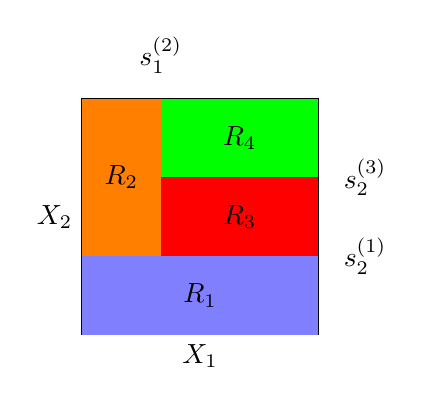
\begin{tikzpicture}
			\draw (0,0)coordinate(A) -- node[below] {$X_1$}  ++ (3,0)coordinate(B) -- (3,3)coordinate(C) -- (0,3)coordinate(D) -- node[left]{$X_2$} cycle;
			
			% initial figure
			\draw[name path=ef] (0,1)coordinate(E) -- (3,1)coordinate(F);
			\draw[name path=gh] (1,1)coordinate(G) -- (1,3)coordinate(H);
			\draw (1,2)coordinate(I) -- (3,2)coordinate(J);
			
			\fill[blue!50](A)--(B)--(F)--(E)--cycle;
			\fill[orange](E)--(G)--(H)--(D)--cycle;
			\fill[red](G)--(F)--(J)--(I)--cycle;
			\fill[green] (I)--(J)--(C)--(H)--cycle;
			
			\node[fill=blue!50,circle,text=black] at (barycentric cs:A=1,B=1,F=1 ,E=1) {$R_1$};
			\node[text=black] at (barycentric cs:E=1,G=1,H=1 ,D=1) {$R_2$};
			\node[text=black] at (barycentric cs:G=1,F=1,J=1 ,I=1) {$R_3$};
			\node[text=black] at (barycentric cs:I=1,J=1,C=1 ,H=1) {$R_4$};	
			
			%split points
			\node[right=0.2cm of F,visible on=<3->]{$s_2^{(1)}$};		
			\node[above=0.2cm of H,visible on=<4->]{$s_1^{(2)}$};
			\node[right=0.2cm of J,visible on=<5->]{$s_2^{(3)}$};
			
						
			%\draw (0, 0) -- node[below]{$X_1$} -- (0, 3)coordinate(B)node[above left]{B} -- (3, 3)coordinate(C)node[above right]{C} -- (3, 0)coordinate(D)node[below right]{D} --cycle;
			%\draw[name path=ae] (B) -- (2, 1)coordinate(E)node[right]{E};
			%\draw[name path=ac] (A) -- (C);
			%\path[name intersections ={of= ae and ac,by=I}];
			%\fill[green](A)--(B)--(I)--cycle;
			%\fill[blue](B)--(C)--(I)--cycle;
			%\fill[red](C)--(E)--(I)--cycle;
			%\fill[violet](A)--(D)--(E)--(I)--cycle;
			\end{tikzpicture}
		\end{column}
	\end{columns}

	
			\visible<2->{\begin{myblock}{Recursive binary splitting}{bg=blue!5,fg=black}{bg=blue!10, fg=black}
				\begin{enumerate}
					\item Start with a constant prediction for all of feature space
					\item Split a leaf-node into two regions (on feature $j$ and split-point $s_j$ chosen by some criteria).
					\item Continue step 2 recursively on all leaves.
				\end{enumerate}
			\end{myblock}
		}
	
\end{frame}

\begin{frame}{Second order gradient tree boosting}
	
	\begin{myblock}{}{bg=blue!5,fg=black}{bg=blue!10, fg=black}
	Iteratively add $\delta f_k$ where $f_k$ are trees trained on derivatives
	\begin{align*}
	g_{ik} =  \left.\frac{\partial}{\partial \pred_i} \loss(\response_i, \pred_i)\right|_{\substack{\pred_i = f^{(k-1)}(\features_i)}}
	\text{ and }
	h_{ik} = \left.\frac{\partial^2}{\partial \pred_i^2} \loss(\response_i, \pred_i)\right|_{\substack{\pred_i = f^{(k-1)}(\features_i)}}.
	\end{align*}
	\end{myblock}
	
		\begin{columns}[T]
		\begin{column}{0.35\textwidth}
			% p0
			\includegraphics<1>[height=4.5cm,width=4.5cm]{figures/tree_boost_p.pdf} 
			\includegraphics<2-4>[height=4.5cm,width=4.5cm]{figures/tree_boost_p_0.pdf}
			%p1
			\includegraphics<5-7>[height=4.5cm,width=4.5cm]{figures/tree_boost_p1.pdf}
			%p2
			\includegraphics<8-10>[height=4.5cm,width=4.5cm]{figures/tree_boost_p2.pdf}			
			%p3
			\includegraphics<11-13>[height=4.5cm,width=4.5cm]{figures/tree_boost_p3.pdf}			
			%p4
			\includegraphics<14>[height=4.5cm,width=4.5cm]{figures/tree_boost_p4.pdf}
		\end{column}
		\begin{column}{0.35\textwidth}
			%res1
			\includegraphics<3>[height=4.5cm,width=4.5cm]{figures/tree_boost_res1.pdf}
			\includegraphics<4-5>[height=4.5cm,width=4.5cm]{figures/tree_boost_resf1.pdf} 
			%res2
			\includegraphics<6>[height=4.5cm,width=4.5cm]{figures/tree_boost_res2.pdf}
			\includegraphics<7-8>[height=4.5cm,width=4.5cm]{figures/tree_boost_resf2.pdf} 
			%res3
			\includegraphics<9>[height=4.5cm,width=4.5cm]{figures/tree_boost_res3.pdf}
			\includegraphics<10-11>[height=4.5cm,width=4.5cm]{figures/tree_boost_resf3.pdf} 
			%res4
			\includegraphics<12>[height=4.5cm,width=4.5cm]{figures/tree_boost_res4.pdf}
			\includegraphics<13-14>[height=4.5cm,width=4.5cm]{figures/tree_boost_resf4.pdf} 
		\end{column}
	\end{columns}

	
\end{frame}

\begin{frame}{Second order gradient tree boosting: Complexity}
	\begin{myblock}{This was too easy!}{bg=blue!5,fg=black}{bg=blue!10, fg=black}
		\begin{itemize}
			\item How do we choose the complexity of the trees?
			\item And how many boosting iterations?
		\end{itemize}
\end{myblock}	
	\begin{columns}[T]
		\begin{column}{0.35\textwidth}
		\includegraphics<2->[height=4.5cm,width=4.5cm]{figures/xgb_boost_p.pdf}			
		\end{column}
		\begin{column}{0.6\textwidth}
			\visible<3->{
			\begin{myblock}{Regularization}{bg=yellow!05,fg=black}{bg=yellow!20, fg=black}
			\begin{itemize}
			\item Choose a maximum depth?
			\item A maximum number of leaf-nodes?
			\item A minimum observations in node?
			\item A minimum reduction in loss when splitting?
			\item A set number of boosting iterations?
			\end{itemize}
			\end{myblock}	
			}
		\end{column}
	\end{columns}
	
\end{frame}


\begin{frame}{The researcher contemplates}
	
	\begin{myblock}{The researcher goes home...}{bg=blue!5,fg=black}{bg=blue!10, fg=black}
		He is determined to win that ML-competition!...
		\begin{itemize}
			\item<2-> But he only has the 2-gb ram laptop running Windows XP that his job graciously gave him as his every-day workhorse.
		\end{itemize}
	\end{myblock}

	\visible<3->{
		
	\begin{columns}[T]
		
		\begin{column}{0.6\linewidth}
			
			\begin{myblock}{So what does he do?}{bg=yellow!05,fg=black}{bg=yellow!20, fg=black}
				\begin{itemize}
					\item<4-> Opt 1: Buy a new computer?
					\item<5-> Opt 2: Expert knowledge on data and tuning?
					\item<6-> Opt 3: Get lucky?
					\item<7-> Opt 4: Rebuild the algorithm to not require tuning?
				\end{itemize}
			\end{myblock}
			
		\end{column}
	
		\begin{column}{0.4\linewidth}
			\visible<8->{
			\begin{myblock}{\small{Plot twist: the researcher is me!}}{bg=green!05,fg=black}{bg=green!20, fg=black}
				\begin{itemize}
					\item<9-> Opt 1: I am a PhD student...
					\item<10-> Opt 2: I am too lazy to be an expert!
					\item<11-> Opt 3: I like good expectations.
					\item<12-> Opt 4: Hmm...
				\end{itemize}
			\end{myblock}
		}
						
		\end{column}

		
	\end{columns}
		
	}
	
\end{frame}

%\subsection{Model complexity selection}

	
\section{An information theoretic approach}

% The problem with increasing complexity
% - Training and test loss as a function of complexity - use trees
% We seek to minimize generalization error
% Most common strategy: cross validation on different input settings
% Goal: Estimate generalization error analytically, by adjusting training error
% Specifically: Estimate generalization error for trees analytically
% Quite generally: 2cov(y_i pred_i)
% So the goal is to estimate cov
% For likelihoods: Akaike - explain Taylor approx?
% Is generalized for differentiable (in parameters) loss functions NIC (Murata)
% Does not apply directly to trees, due to the non-standard binary splitting procedure
% However, conditioned on topology. Only leaf-parameters are learned (satisfies differentiability etc.) - local optimism as NIC
% Big result - 

\begin{frame}{Revisit the supervised learning problem}
	The goal is to find $f$ that minimises \textit{generalization error}:
	\begin{align*}
	\hat{f} = \arg\min_f E_{\hat{\theta},\features^0\response^0}\left[l(\response^0,f(\features^0;\hat{\theta}))\right]
	\end{align*}
	where $(\features^0\response^0)$ are unseen in the training-phase, and therefore independent of $\hat{\theta}$ trained from $(\features,\response)$.
	
	\begin{columns}[T]
		\begin{column}{0.35\textwidth}
		\includegraphics<2->[height=4.5cm,width=4.5cm]{figures/loss_vs_complexity.pdf}			
		\end{column}
		\begin{column}{0.6\textwidth}
			\visible<3->{
			\begin{myblock}{}{bg=yellow!05,fg=black}{bg=yellow!20, fg=black}
				\begin{itemize}
					\item<1-> Optimism of the training loss: \small$$C(\hat{\theta}) = E\left[l(\response^0,f(\features^0;\hat{\theta})) - l(\response,f(\features;\hat{\theta}))\right]$$
					\item<1-> Often \small$C(\hat{\theta})\approx \frac{2}{n}\sum_{i=1}^n\Cov(y_i,\pred_i)$
					\item<1-> Useful to talk about \textit{asymptotic loss} \small$$E\left[l(\response,f(\features;\theta_0))\right],~\lim_{n\to\infty}\hat{\theta}\stackrel{P}{\to}\theta_0$$
				\end{itemize}
			\end{myblock}}
		\end{column}
	\end{columns}
	
	
%	The goal is to find $f$ that minimizes generalization error:
%	
%	where XXX is data unseen in the training-phase.
%	
%	Training and test error on as a function of complexity
%	
%		Optimism definition
%	
%	Then add asymptotic one
%	
%	The general result with cov
	
	
\end{frame}

\begin{frame}{But the ensemble complexity is unknown...}
	
	\begin{myblock}{The main idea:}{bg=green!05,fg=black}{bg=green!20, fg=black}
		\begin{itemize}
			\item<1-> Estimate $C(\hat{\theta})$ for trees analytically!
		\end{itemize}
	\end{myblock}
	
	\begin{myblock}{And hope that we may...}{bg=yellow!05,fg=black}{bg=yellow!20, fg=black}
		\begin{enumerate}
			\item<2-> Adaptively control the complexity of each tree
			\item<3-> Automatically stop the boosting procedure
			%\item<4-> In a highly efficient manner
		\end{enumerate}
	\end{myblock}
	\begin{columns}[T]
	\begin{column}{0.35\textwidth}
		% tree loss vs depth
		\includegraphics<2->[height=4cm,width=4.5cm]{figures/loss_vs_treedepth1.pdf} 
	\end{column}
	\begin{column}{0.35\textwidth}
		% no split at all
		\includegraphics<3>[height=4cm,width=4.5cm]{figures/loss_vs_treedepth2.pdf}
	\end{column}
	\end{columns}
	
\end{frame}

\begin{frame}{Information criteria: Akaike and beyond...}
	\begin{myblock}{The poor researcher has no processing power...}{bg=blue!5,fg=black}{bg=blue!10, fg=black}
		\begin{itemize}
			\item<1-> An analytic, not a data-driven approach, is needed!
		\end{itemize}
	\end{myblock}
	\visible<2->{\begin{myblock}{A brief history of (some) information criteria}{bg=yellow!05,fg=black}{bg=yellow!20, fg=black}
		\begin{itemize}
			\item<2-> \cite{akaike1974new} AIC: $C=p$ for NLL. Assumptions on true model
			\item<2-> \cite{takeuchi1976distribution} TIC: $C = \tr(QH^{-1})$ also for NLL, but no assumption on the true model
			\item<2-> \cite{murata1994network} NIC: $C = \tr(QH^{-1})$ also for differentiable loss
		\end{itemize}
		\begin{align*}
	H&=\E \left[ \nabla_{\mathbf{\theta}_0}^2 \loss(\response,f(\features;\mathbf{\theta}_0)) \right]\\ 
	Q &= \E\left[ \left( \nabla_{\theta_0}\loss(\response,f(\features;\mathbf{\theta}_0)) \right)\left( \nabla_{\theta_0}\loss(\response,f(\features;\mathbf{\theta}_0)) \right)^\intercal  \right]
	\end{align*}
	\end{myblock}
}
	%Yellow block local optimism conditioning?
\end{frame}

\begin{frame}{The local optimism}
	
				\begin{myblock}{But can we use this for trees?}{bg=blue!5,fg=black}{bg=blue!10, fg=black}
				\begin{itemize}
					\item<2-> Conditionally on known tree-topology / regions $R$
					\item<2-> We define the local optimism for a leaf node $t$
					\begin{align*}
						\mathcal{C}(t|q) &= 
						\E_{y,\hat{w}_t} \left[ \frac{\partial^2}{\partial \hat{w}_t^2}\tilde l(\response,\hat{w}_t)\right]
						\Var_{\hat{w}_t}[\hat{w}_{t}]
					\end{align*}
					$q$ is the tree-topology, $\hat{w}_t$ is the prediction in region $t$
				\end{itemize}
			\end{myblock}
		
		\visible<3->{
	\begin{myblock}{Correspondingly for internal nodes...}{bg=yellow!05,fg=black}{bg=yellow!20, fg=black}
		\begin{itemize}
			\item<3-> At some stage in the tree building process every node will have been a leaf node.
			\item<3-> Define this to be the local optimism $\mathcal{C}(t|q)$ for the internal node $t$ in the fully grown tree.
		\end{itemize}
	\end{myblock}	
	}			

\end{frame}

\begin{frame}{The local optimism: Illustration}
	\centering\resizebox{7cm}{4cm}{
		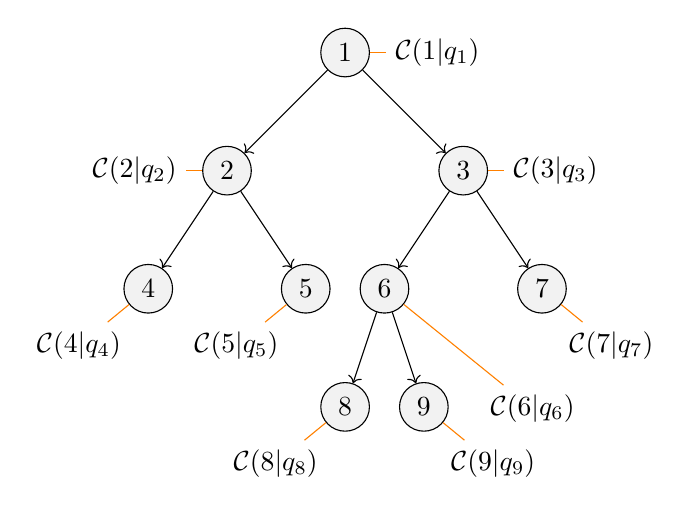
\begin{tikzpicture}
\tikzstyle{custbox} = [circle, align=left, minimum width=0.5cm, minimum height=0.5cm,text centered, draw=black, fill=gray!10]

\node (r) at (0,0) [custbox]{1}; 
\node[right=0.2cm of r] (optimismr) {$\mathcal{C}(1|q_1)$};

\node (rl) at (-1.5,-1.5) [custbox]{2}; 
\node[left=0.2cm of rl] (optimismrl) {$\mathcal{C}(2|q_2)$};

\node (rll) at (-2.5,-3) [custbox]{4}; \node[below left=0.2cm and 0cm of rll] (opt4) {$\mathcal{C}(4|q_4)$}; 
\node (rlr) at (-0.5,-3) [custbox]{5}; \node[below left=0.2cm and 0cm of rlr] (opt5) {$\mathcal{C}(5|q_5)$}; 

\node (rr) at (1.5,-1.5) [custbox]{3};
\node[right=0.2cm of rr] (optimismrr) {$\mathcal{C}(3|q_3)$};

\node (rrl) at (0.5,-3) [custbox]{6};
\node[below right=1cm and 1cm of rrl] (optimismrrl) {$\mathcal{C}(6|q_6)$};

\node (rrll) at (0,-4.5) [custbox]{8}; \node[below left=0.2cm and 0cm of rrll] (opt8) {$\mathcal{C}(8|q_8)$}; 
\node (rrlr) at (1,-4.5) [custbox]{9}; \node[below right=0.2cm and 0cm of rrlr] (opt9) {$\mathcal{C}(9|q_9)$}; 
\node (rrr) at (2.5,-3) [custbox]{7}; \node[below right=0.2cm and 0cm of rrr] (opt7) {$\mathcal{C}(7|q_7)$}; 

%Arrows
\draw[->,black] (r) -- (rl);
\draw[->,black] (r) -- (rr);
\draw[->,black] (rl) -- (rll);
\draw[->,black] (rl) -- (rlr);
\draw[->,black] (rr) -- (rrl);
\draw[->,black] (rr) -- (rrr);
\draw[->,black] (rrl) -- (rrll);
\draw[->,black] (rrl) -- (rrlr);
%optimism
\draw[-,orange] (r) -- (optimismr);
\draw[-,orange] (rr) -- (optimismrr);
\draw[-,orange] (rrl) -- (optimismrrl);
\draw[-,orange] (rl) -- (optimismrl);
\draw[-,orange] (rll) -- (opt4);
\draw[-,orange] (rlr) -- (opt5);
\draw[-,orange] (rrr) -- (opt7);
\draw[-,orange] (rrll) -- (opt8);
\draw[-,orange] (rrlr) -- (opt9);


\end{tikzpicture}
}

The optimism induced from fitting the predictions $\mathbf{w}$ in the leaf-nodes conditioned on the final topology is given as
\begin{align*}
	\hat{C}(\hat{\mathbf{w}}|q) = \sum_{t\in\{4,5,8,9,7\} } \mathcal{C}(t|q)\pi_t,~\pi_t=P(q(\mathbf{x})=t)
\end{align*}

\end{frame}


\begin{frame}{The tree-learning procedure learns the future map $q$}
	\begin{myblock}{The steps - first consider only one feature}{bg=blue!5,fg=black}{bg=blue!10, fg=black}
	\begin{itemize}
		\item<1-> Relate the distance between the training and asymptotic loss to a gamma distribution
		\item<1-> Fit the gamma using knowledge of its shape and expectation
	\end{itemize}
	\end{myblock}
\visible<2->{
	\begin{myblock}{The steps - consider $m\geq 1$ features}{bg=yellow!05,fg=black}{bg=yellow!20, fg=black}
		\begin{itemize}
			\item<2-> Under $H_0$: no feature is relevant
			\item<2-> Distance between training and asymptotic loss as expected maximum of multiple realizations of the gamma RV
		\end{itemize}
	\end{myblock}	
}	
\begin{itemize}
	\item<2-> Warning: several approximations!
\end{itemize}
\end{frame}

\begin{frame}{Gives the following result:}
	\begin{align*}
	\hat{C}_m(\hat{\mathbf{w}}, q) 
	=
	2 \sum_{t\not\in \mathcal{L}} \E \left[
	Q\left(
	d(t), \frac{ \mathcal{C}(L(t)|q)\pi_{L(t)} + \mathcal{C}(R(t)|q)\pi_{R(t)} }{2}, m
	\right)
	\right]
	\end{align*}
	\begin{itemize}
		\item $\mathcal{L}$ is the set of leaf nodes
		\item $Q(\alpha,\beta,m)$ is the maximum of $m$ gamma random variables with shape $\alpha$ and scale $\beta$
		\item $L(t)$ and $R(t)$ returns the index of left and right child-nodes respectively
		\item 	\small\begin{align*}
		d(t) = 
		\begin{cases}
		3 & \text{if } L(t) \in \setleafnodes \text{ and } R(t) \in \setleafnodes\\
		\frac{5}{2} & \text{if } L(t) \in \setleafnodes \text{ and } R(t) \not\in \setleafnodes\\
		\frac{5}{2} & \text{if } L(t) \not\in \setleafnodes \text{ and } R(t) \in \setleafnodes\\
		2 & \text{if } L(t) \not\in \setleafnodes \text{ and } R(t) \not\in \setleafnodes.
		\end{cases}
		\end{align*} 
	\end{itemize}
\end{frame}

\begin{frame}{Visualization of the result}
	\centering\resizebox{11cm}{4.5cm}{
	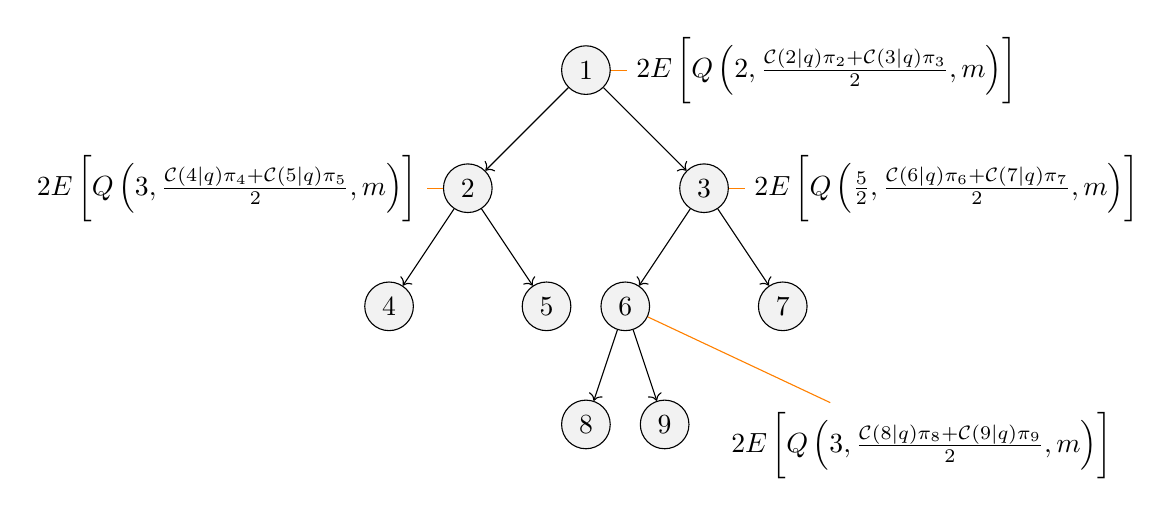
\begin{tikzpicture}
	\tikzstyle{custbox} = [circle, align=left, minimum width=0.5cm, minimum height=0.5cm,text centered, draw=black, fill=gray!10]
	
	\node (r) at (0,0) [custbox]{1}; 
	\node[right=0.2cm of r] (optimismr) {$2E\left[Q\left(2,\frac{\mathcal{C}(2|q)\pi_2+\mathcal{C}(3|q)\pi_3}{2}, m\right)\right]$};
	
	\node (rl) at (-1.5,-1.5) [custbox]{2}; 
	\node[left=0.2cm of rl] (optimismrl) {$2E\left[Q\left(3,\frac{\mathcal{C}(4|q)\pi_4+\mathcal{C}(5|q)\pi_5}{2}, m\right)\right]$};
	
	\node (rll) at (-2.5,-3) [custbox]{4}; %\node[below=0.2cm of rll] {$\hat{w}_1$}; 
	\node (rlr) at (-0.5,-3) [custbox]{5}; %\node[below=0.2cm of rlr] {$\hat{w}_2$}; 
	
	\node (rr) at (1.5,-1.5) [custbox]{3};
	\node[right=0.2cm of rr] (optimismrr) {$2E\left[Q\left(\frac{5}{2},\frac{\mathcal{C}(6|q)\pi_6+\mathcal{C}(7|q)\pi_7}{2}, m\right)\right]$};
	
	\node (rrl) at (0.5,-3) [custbox]{6};
	\node[below right=1cm and 1cm of rrl] (optimismrrl) {$2E\left[Q\left(3,\frac{\mathcal{C}(8|q)\pi_8+\mathcal{C}(9|q)\pi_9}{2}, m\right)\right]$};
	
	\node (rrll) at (0,-4.5) [custbox]{8};% \node[below=0.2cm of rrll] {$\hat{w}_3$}; 
	\node (rrlr) at (1,-4.5) [custbox]{9};% \node[below=0.2cm of rrlr] {$\hat{w}_4$}; 
	\node (rrr) at (2.5,-3) [custbox]{7}; %\node[below=0.2cm of rrr] {$\hat{w}_5$}; 
	
	%Arrows
	\draw[->,black] (r) -- (rl);
	\draw[->,black] (r) -- (rr);
	\draw[->,black] (rl) -- (rll);
	\draw[->,black] (rl) -- (rlr);
	\draw[->,black] (rr) -- (rrl);
	\draw[->,black] (rr) -- (rrr);
	\draw[->,black] (rrl) -- (rrll);
	\draw[->,black] (rrl) -- (rrlr);
	%optimism
	\draw[-,orange] (r) -- (optimismr);
	\draw[-,orange] (rr) -- (optimismrr);
	\draw[-,orange] (rrl) -- (optimismrrl);
	\draw[-,orange] (rl) -- (optimismrl);
	
	\end{tikzpicture}
}
	\begin{itemize}
	\item Sum up the node-contributions to obtain the optimism estimate
	\end{itemize}
\end{frame}

\begin{frame}{Estimation}
	Quantities must admit evaluation and efficient computation:
	\begin{itemize}
		\item<2-> Conditioned on $q$, $\hat{\mathbf{w}}$ are M-estimators.
		\item<2-> 	\begin{align*}
		\lim_{n\to\infty}
		\mathcal{C}(t|q)\pi_t
		&=
		\E_{y,\hat{w}_t} \left[ \frac{\partial^2}{\partial \hat{w}_t^2}l(\response,\hat{w}_t)\right]
		\Var_{\hat{w}_t}[\hat{w}_{t}]\pi_t\\
		%,~t\in\setleafnodes,~q(\features)=t\\
		&= 
		\frac{\sum_{i\in I_t} \left(g_i+h_i\hat{w}_t\right)^2}{n\sum_{i\in I_t}h_i},
		\text{ $I_t$ is indexes of obs in leaf $t$}
		\end{align*}
		\item<3-> Assume features independent, then $E[Q]$ is the expected $m-$th order statistic
		\item<3-> Estimate asymptotically using the gamma-quantile function: $$E[Q]\sim z\left(\frac{m}{m+1}\right)$$
	\end{itemize}
\end{frame}

\begin{frame}{Some sanity checks: Simulation experiments}
	
	100 Datasets and 100 trees, trained on 1 and 100 features.
		\begin{figure}[h]
		\centering
		\begin{subfigure}{.43\textwidth}
			\centering
			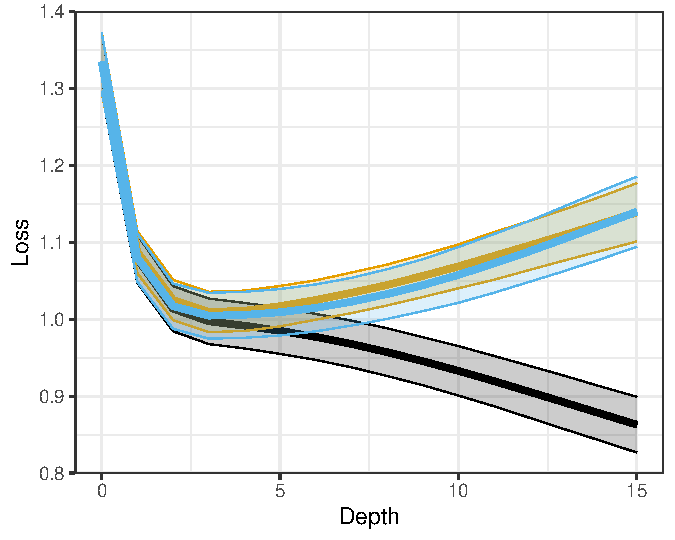
\includegraphics[scale=0.4]{figures/loss_vs_depth_one_feature.pdf}
			\caption[]{One (relevant) feature}
			\label{fig: loss vs tree depth one feature}
		\end{subfigure}
		\begin{subfigure}{.53\textwidth}
			\centering
			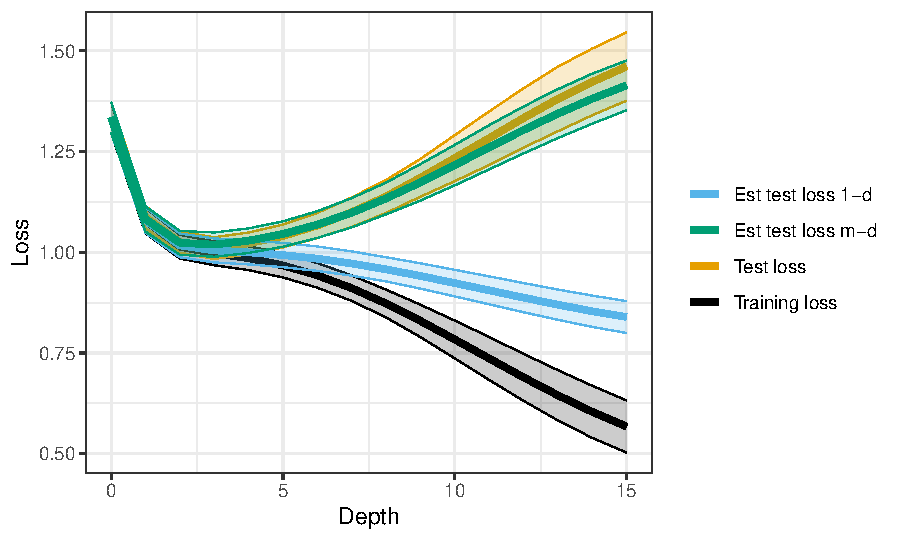
\includegraphics[scale=0.4]{figures/loss_vs_depth_dim_correct.pdf} 
			\caption[]{100 features of which 99 are noise}
			\label{fig: loss vs tree depth multiple feature}
		\end{subfigure}
	\caption{Average $\pm 2 SD$ for training (black) and test (orange) MSE loss, together with estimated optimism (blue: 1 feature, green: 100 features)}
		%\caption{The average $\pm 2 SD$ for training (black) and test (orange) MSE loss, and estimated optimism, after training on 100 simulated datasets, each containing 10000 realizations from a linear model $y\sim N(x,1)$ where $x\sim U(0,2)$. In Figure (a), training is done on only one feature (the relevant $x$), and the quantity \eqref{eq:expected tree optimism one feature} (blue) is the optimism added to the training loss. Figure (b) results from the same data and training, but with 99 added Gaussian noise features. Resulting is that the optimism from Figure (a) is pushed downwards, and in need of the correction given in \eqref{eq:optimism full m} (green). }
	\end{figure}
	\begin{itemize}
		\item<2-> Not crazy!
	\end{itemize}
\end{frame}

\section{Applications to the boosting algorithm}

\begin{frame}{Going back to the original idea}
	
	
	\begin{myblock}{Our hope was to...}{bg=yellow!05,fg=black}{bg=yellow!20, fg=black}
		\begin{enumerate}
			\item<1-> Adaptively control the complexity of each tree
			\item<1-> Automatically stop the boosting procedure
			%\item<4-> In a highly efficient manner
		\end{enumerate}
	\end{myblock}
	
	\visible<2->{
	\begin{myblock}{What we do: Two inequalities}{bg=green!05,fg=black}{bg=green!20, fg=black}
	\begin{enumerate}
		\item<2-> For two hierarchical trees, $q^0$ and $q^1$, where $q^1$ holds one more split than $q^0$, don't split if
		\begin{align*}
		\E\left[\hat{l}(\response,f(\features;\hat{\mathbf{w}}^0,\hat{q}^0)) - \hat{l}(\response,f(\features;\hat{\mathbf{w}}^1,\hat{q}^1))\right] + C_m(\hat{\mathbf{w}}^0,\hat{q}^0)
		 - C_m(\hat{\mathbf{w}}^1,\hat{q}^1)
		\end{align*}
		is smaller than zero.
		\item<3-> Stop the iterative boosting algorithm when
		\begin{align*}
		\frac{\delta\left(\delta - 2\right)}{2n}  \sum_{t\in\setleafnodes_k}\frac{G_{tk}^2}{H_{tk}}
		+ \delta C_m\left(\hat{\mathbf{w}}_{t,k},q_{t,k}\right) > 0.
		\end{align*}
	\end{enumerate}
	\end{myblock}
}

	
\end{frame}

\begin{frame}{The algorithm}
%	\resizebox{10cm}{8cm}{
	\small\begin{tabbing}
	\hspace{2em} \= \hspace{2em} \= \hspace{2em} \= \\
	{\bfseries Input}: \\
	\> - A training set $\data_n=\{(x_i, y_{i})\}_{i=1}^n$,\\
	\> - a differentiable loss $l(y,f(x))$,\\
	\> - a learning rate $\delta$,\\
	\> \colorbox{blue!20}{- boosting iterations $K$},\\
	\> \colorbox{blue!20}{- one or more tree-complexity regularization criteria.}\\
	
	1. Initialize model with a constant value:
		$f^{(0)}(\features) = \hat{\eta}= \underset{\eta}{\arg\min} \sum_{i=1}^n \loss(y_i, \eta).$\\
	
	2. \colorbox{blue!20}{{\bfseries for} $k = 1$ to $K$:} \colorbox{orange!30}{{\bfseries while} the inequality (2) evaluates to \textbf{\texttt{false}} } \\
	
	\>	$i)$ Compute derivatives $g_i$ and $h_i$ for all $i=1:n$.\\
	
	\> $ii)$ Determine $q_k$ by the iterative binary splitting procedure until\\
	\>\> \colorbox{blue!20}{a regularization criterion is reached.} \colorbox{orange!30}{ the inequality (1) is \textbf{\texttt{true}} }\\ 
	
	\> $iii)$ Fit the leaf weights $\mathbf{w}$, given $q_k$\\
	
	\>	$v)$ Update the model with a scaled tree:
		$f^{(k)}(\features) = f^{(k-1)}(\features) + \delta f_k(\features).$\\
	{\bfseries end \colorbox{blue!20}{for} \colorbox{orange!30}{while}}\\
	
	3. Output the model: {\bfseries Return} $f^{(K)}(\features)$.%=\sum_{k=0}^{K}f_k(\features)$.\\
	
\end{tabbing}

\end{frame}

\begin{frame}{Does it work?}
	
	\begin{itemize}
		\item The tree-boosting animation in the introduction was generated by this algorithm.
	\end{itemize}
\visible<2->{
	\begin{figure}
		\centering
		\includegraphics<2->[height=4.5cm,width=7cm]{figures/loss_vs_numtrees.pdf}			
		\caption{Training (black) and test loss (orange) and estimated generalization error (blue), for a tree-boosting ensemble trained on 1000 observations from a linear model: $\response\sim N(\features, 1)$. The blue line visualizes inequality 2.}
	\end{figure}
	}
\end{frame}


\begin{frame}{ISLR and ESL datasets}
	
	\begin{itemize}
		\item Comparisons on real data
		\item Every dataset randomly split into training and test datasets 100 different ways
		\item Average test scores (relative to XGB) and standard deviations (parenthesis) 
	\end{itemize}
		
\centering\resizebox{10cm}{2cm}{		
		\begin{tabular}{@{\extracolsep{4pt}}lcccccc} 
		\\[-1.8ex]\hline 
		\hline \\[-1.8ex] 
		Dataset & \multicolumn{1}{c}{Dimensions} & \multicolumn{1}{c}{GBTorch} &  \multicolumn{1}{c}{GLM} & \multicolumn{1}{c}{Random forest} & \multicolumn{1}{c}{XGBoost} \\ 
		\hline \\[-1.8ex] 
		Boston  & $506 \times 14$  & 1.07 (0.162)  &  1.3 (0.179)  & 0.876 (0.15)  & 1 (0.176)   \\  
		Ozone  & $111\times 4$  &0.827 (0.22)  &  0.666 (0.131)  & 0.669 (0.182)  & 1 (0.202)   \\  
		Auto  & $392\times 311$  &1.16 (0.136)  &  11.1 (14.5)  & 0.894 (0.134)  & 1 (0.188)   \\  
		Carseats  &  $400\times 12$  & 1.2 (0.168)  &  0.413 (0.0432)  & 1.16 (0.141)  & 1 (0.115)   \\  
		College   & $777\times 18$& 1.3 (0.948)  & 0.55 (0.154)  & 1.07 (0.906)  & 1 (0.818)   \\  
		Hitters   & $263\times 20$ & 1.05 (0.362)  &  1.21 (0.347)  & 0.796 (0.31)  & 1 (0.318)   \\  
		Wage  & $3000\times 26$ & 1.96 (1.72)  &  289 (35.4)  & 82.2 (21.3)  & 1 (1.01)   \\ 
		Caravan  & $5822\times 86$ & 1.02 (0.0508) & 1.12 (0.115)  & 1.31 (0.168)  & 1 (0.0513)   \\  
		Default  & $10000\times 4$ & 0.938 (0.068)  & 0.902 (0.0698)  & 2.83 (0.51)  & 1 (0.0795)   \\  
		OJ  & $1070\times 18$ & 0.996 (0.0496)  & 0.952 (0.0721)  & 1.17 (0.183)  & 1 (0.0703)   \\  
		Smarket  & $1250\times 7$ & 0.999 (0.00285)  &  1 (0.00651)  & 1.04 (0.0164)  & 1 (0.00259)   \\  
		Weekly  & $1089\times 7$	 & 0.992 (0.0082)  &  0.995 (0.0123)  & 1.02 (0.0195)  & 1 (0.00791)   \\  
		\hline \\[-1.8ex] 
	\end{tabular} 
}
\end{frame}

\begin{frame}{Computational considerations}
	
	\begin{myblock}{In general...}{bg=yellow!05,fg=black}{bg=yellow!20, fg=black}
	\begin{itemize}
		\item Let $k$-fold cross validation be used to determine the tuning for a standard tree-boosting implementation using "early-stopping".
		\item Consider $p$ hyperparameters, each having $r$ candidate values.
		\item<1-> Then our implementation is approximately $k\times r^p +1 $ times faster.
	%	\item<2-> Should give similar results to $p=4$ (tree-complexity criteria).
	\end{itemize}
	\end{myblock}
\visible<2->{
	\begin{myblock}{A comparison with XGB}{bg=green!05,fg=black}{bg=green!20, fg=black}
		\begin{itemize}
			\item<2-> On the Caravan dataset ($5822\times 86$ classification), our implementation took 2.68 seconds to train.
			\item<3-> Using a 30\% validation set, XGB took 4.85 seconds
			\item<4-> One minute using $10$-fold CV: the number of boosting iterations
			\item<5-> About 16 minutes to learn one additional hyperparameter
			\item<6> About 2.65 hours on yet another additional hyperparameter
		\end{itemize}
	\end{myblock}
	}
\end{frame}


% LAST SLIDE in Applications
\begin{frame}{The researcher enters the ML competition}
	
	\begin{itemize}
		\item Would he win?
	\end{itemize}

\visible<2->{
	\begin{myblock}{There are additional techniques for improvement}{bg=blue!5,fg=black}{bg=blue!10, fg=black}
	Most notably...
	\begin{itemize}
	%	\item<2-> Most notably...
		\item<3-> L1-L2 regularization
		\item<3-> Stochastic sampling of both rows and columns
		\item<3-> Our trees are optimal if they all were the last (unscaled) tree
	\end{itemize}
	\end{myblock}
	}
\visible<4->{
	\begin{myblock}{But there are benefits!}{bg=yellow!05,fg=black}{bg=yellow!20, fg=black}
		%But he would have an advantage
		\begin{itemize}
			\item The key to many ML competitions is the feature engineering
			\item Possibility of very quickly (and automatically) testing for relevant features
		\end{itemize}
	\end{myblock}
}
\end{frame}

\section{Implementation and notes on future developments} 
% gbtorch project
% automatic and adaptive deterministic frequentist GTB
% Optimal and automatic deterministic frequentist GTB
% Optimal and automatic deterministic GTB
% Optimal and automatic GTB (goal)
% works as a summary and why I am excited


\begin{frame}[fragile]{GBTorch package}
	\begin{itemize}
		\item Algorithm implemented in the \texttt{GBTorch} project on Github: \url{https://github.com/Blunde1/gbtorch}
		\item Install the \texttt{R}-package from GitHub:
		\begin{lstlisting}[language=R]
		devtools::install_github("Blunde1/gbtorch/R-package")
		\end{lstlisting}
		\item Implemented in \texttt{C++}, depends upon \texttt{Eigen} for linear algebra
		\item Depends on \texttt{Rcpp} for the \texttt{R}-package
		\item<2-> Designed to be super easy:
		\begin{lstlisting}[language=R]
			x <- runif( 500, 0, 4 )
			y <- rnorm( 500, x, 1 )
			x.test <- runif( 500, 0, 4 )
			y.test <- rnorm( 500, x.test, 1 )
			# Train gbtorch ensemble
			mod <- gbt.train( y, as.matrix(x) )
			y.pred <- predict( mod, as.matrix( x.test ) )
			# Plot predictions on test data
			plot( x.test, y.test )
			points( x.test, y.pred, col="red" )
		\end{lstlisting}
	\end{itemize}
	
\end{frame}

\begin{frame}{Future development \#1}
	
	\small\begin{myblock}{There are additional techniques for improvement}{bg=blue!5,fg=black}{bg=blue!10, fg=black}
		Most notably...
		\begin{itemize}
			%	\item<2-> Most notably...
			\item<1-> L1-L2 regularization
			\item<1-> Stochastic sampling of both rows and columns
			\item<1-> \colorbox{red!20}{Our trees are optimal if they all were the last (unscaled) tree}
		\end{itemize}
	\end{myblock}

	

	\begin{myblock}{Solved!}{bg=green!05,fg=black}{bg=green!20, fg=black}
		\begin{itemize}
		\item Philosophy from LARS / FS\_0: Only add as much complexity in a certain direction as it deserves...
		\item Modifies the standard greedy recursive binary splitting procedure...
		\item Implemented in GBTorch: \colorbox{yellow}{\lstinline[language=R]{gbt.train(y, x, greedy_complexities=T)}}
		\item Better results than XGB on ISLR / ESL data!
		
		0.941 0.794 1.02 0.984 1.1 0.975 0.989 0.996 0.914 0.964 0.998 0.991
	\end{itemize}

	\end{myblock}

	%smarket funny mention
\end{frame}

\begin{frame}{Future development \#2}
	
	\begin{myblock}{There are additional techniques for improvement}{bg=blue!5,fg=black}{bg=blue!10, fg=black}
	
		Most notably...
		\begin{itemize}
			%	\item<2-> Most notably...
			\item<1-> \colorbox{red!20}{L1-L2 regularization}
			\item<1-> Stochastic sampling of both rows and columns
			\item<1-> Our trees are optimal if they all were the last (unscaled) tree
		\end{itemize}
	\end{myblock}
\visible<1->{
	\begin{myblock}{Hmm!}{bg=green!05,fg=black}{bg=green!20, fg=black}
	\begin{itemize}
		\item Can we automatically tune this?
		\item Weights, $\mathbf{w}$ resulting from a L-2 regularized objective are still M-estimators... 
	\end{itemize}
	\end{myblock}}
\end{frame}

\begin{frame}{Future development \#2}
		Around Christmas 2018 I was thinking about this problem in general: %Is it possible to do gradient descent on L1-L2 regularization parameters for a typical...
		\begin{itemize}
			\item Given trainin data, how can we automatically know how strongly we should believe in a prior about some $H_0$?
		\end{itemize}
		\begin{myblock}{Solution}{bg=green!05,fg=black}{bg=green!20, fg=black}
		\begin{itemize}
			\item Create an information criterion, taking into account the alternation between the regularized and un-regularized objectives.
			\item Make it differentiable...
			\item Gradient descent: $\nabla_\lambda \left[ l(y,f(x;\hat{\theta}(\lambda))) + \tr(Q(\lambda)H(\lambda)^\intercal) \right]$
			%\item Extremely computationally expensive... but works:
		\end{itemize}
		\end{myblock}
	%c
	
		
		
%			Alternating objectives criterion
%		Gradient descent on $\lambda$ belief in prior!
%		Ridge implementation
%		But very computationally costly: grad of trace hessian...
%		
%		What is locally constant and the building block of our method?... 
%		Another quantile: log loglog..
	
\end{frame}

\begin{frame}{Future development \#2}
	
%	\begin{itemize}
%	\item Gradient descent: $\nabla_\lambda \left[ l(y,f(x;\hat{\theta}(\lambda))) + \tr(Q(\lambda)H(\lambda)^\intercal) \right]$
%	\end{itemize}
	\begin{figure}
				\caption{	Hitters data: dimensions $263\times 20$}
		\centering
		\includegraphics<1->[height=3.5cm,width=7cm]{figures/grad_altobj.pdf}			
	\end{figure}
	\begin{itemize}
		%\item Test error for ridge regression trained with our approach and CV in GLMNET, and ordinary linear regression. 
			\item Gradient descent: $\nabla_\lambda \left[ l(y,f(x;\hat{\theta}(\lambda))) + \tr(Q(\lambda)H(\lambda)^\intercal) \right]$
		\item Equivalent results to GLMNET for ridge regression.
		\item Extremely computationally expensive... 
		\item<2-> But, what is locally constant and the base-learners of choice?
	\end{itemize}



\end{frame}


\begin{frame}{We could make this even better!}
	
	When this project has matured... 
	\begin{myblock}{any help on the following subjects are welcome:}{bg=yellow!05,fg=black}{bg=yellow!20, fg=black}
			\begin{itemize}
			\item Utilizing sparsity (possibly Eigen sparsity)
			\item Parallelisation (CPU and/or GPU)
			\item Distribution (Python, Java, Scala, ...)
			\end{itemize}
	\end{myblock}

	
\end{frame}





\begin{frame}
\frametitle{Conclusion}
		
	\begin{columns}[T]
		\begin{column}{0.48\textwidth}
	\begin{myblock}{Work being done}{bg=blue!5,fg=black}{bg=blue!10, fg=black}
	\begin{itemize}
		\item Writing a paper on the work presented
		\item Robustness of theory
		\item Will continue development after submission
		\item And write more papers on future developments
	\end{itemize}
	\end{myblock}
		\end{column}
	\visible<2->{
	\begin{column}{0.48\textwidth}
			\begin{myblock}{Why I'm excited}{bg=green!05,fg=black}{bg=green!20, fg=black}
			\begin{itemize}
				\item Tree-boosting is very popular!
				\item Removing manual tuning may potentially help quite a few people...
				\item and opens up for new applications
				\item Training a highly competitive model will be computationally trivial
			\end{itemize}
		\end{myblock}
	\end{column}
}
	\end{columns}
		
\end{frame}


\begin{frame}{Bibliography}
	\bibliographystyle{apalike}
	\scriptsize\bibliography{Bibliography}   % name your BibTeX data base
\end{frame}



\end{document}


